
\section{Experimental verification of Reactive Collision Avoidance}
The Stack of Tasks (SoT) controller with collision avoidance constraints has also been deployed and tested for achieving different postures on the setup in Fig. \ref{fig:TUDSetup}. We have integrated the behavior to path following with the reactive collision avoidance as shown in Fig. \ref{fig:dca}. Though it is integrated, we consider these presented results preliminary yet quite convincing to be go in this direction to develop a reactive collision avoidance technology.

\subsection{Experiments in a mobile robot - PR2{\color{red}  (to be updated)}}

The framework was very initially tested with the given skin cell prototype on PR2, a mobile robot. The skin patch with eight cells is stuck on the arm to sense proximity range information. A simple manipulation scenario is executed and getting close to the arm sensors induced base motion to avoid obstacles while still executing the trajectory. The experiment can be seen here in this \href{https://youtu.be/y-6Oyi21ioQ}{\textcolor{blue}{video}} and the snapshots are shown in this Fig \ref{fig:pr2avoid}. The graph \ref{fig:basegraph} shows the evolution of the robot base when it encounters an obstacle. The safe region is where the skin cell - obstacle distance is within the right limits ensuring safety. Although the base goes away from the obstacle, it recovers back to its previous or commanded pose in the trajectory. 
\begin{figure}[ht]
\centering
\begin{subfigure}
[Getting close to the arm]{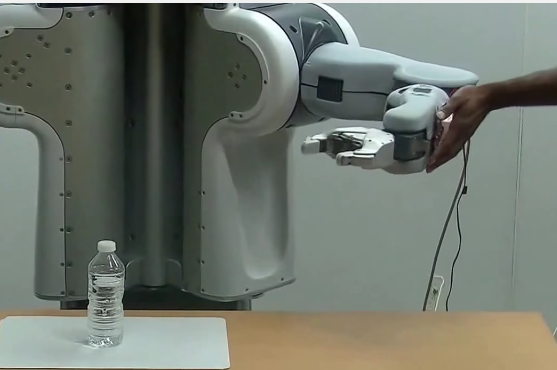
\includegraphics[width=5.5cm,height=6cm]{chapters/doa/images/pr2_0.png}}
\end{subfigure}
\begin{subfigure}
[Base motion to avoid the obstacle]{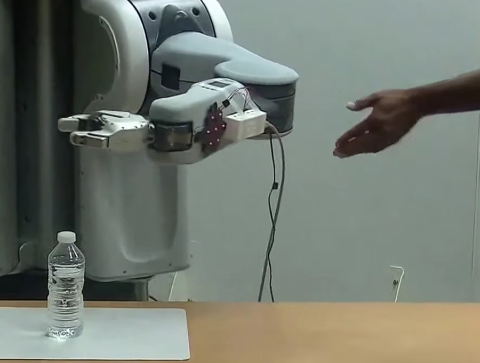
\includegraphics[width=5.5cm,height=6cm]{chapters/doa/images/pr2_1.png}}
\end{subfigure}
\caption{Obstacle Avoidance in PR2 using skin prototype}
\label{fig:pr2avoid}
\end{figure}

\begin{figure}[!ht]
\centering
{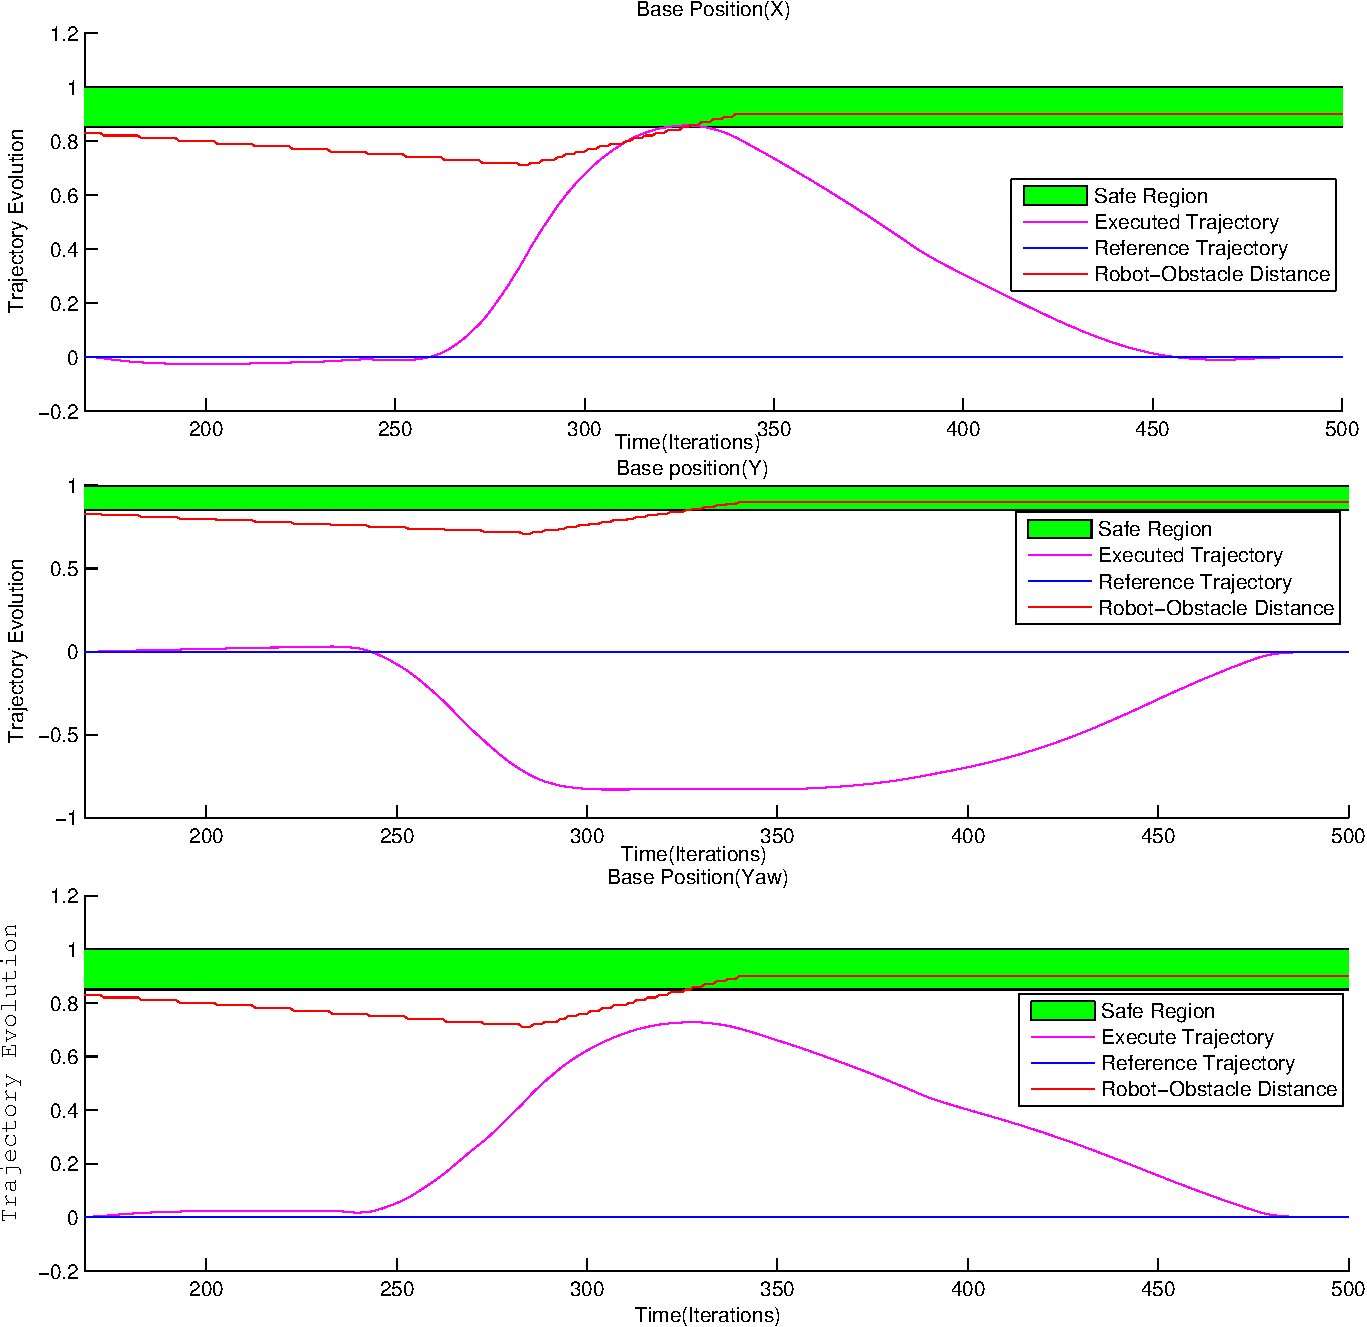
\includegraphics[scale=0.5]{chapters/doa/images/baseplot-crop.pdf}}
\caption{Base Position Evolution}
\label{fig:basegraph}
\end{figure}




\subsection{Experiments with Reactive Replanning in TOMM Setup}
\hypersetup{colorlinks, linkcolor=blue}
The integration of all the components described earlier has been evaluated on a simulation of the orange sorting setup as shown in Fig. \ref{fig:TOMMSimulation}. The evaluation is done in a ROS based gazebo environment with the skin sensors simulated using the flexible collision library to project the distance between objects to sensor range measurements. These measurements are mapped to signals compatible in dynamic graph framework using a bridge component to allow its use in the SoT controller. The reactive planning component having the capability to plan with point cloud data using a Moveit python interface to query motion plan requests. 
\begin{figure}[ht]
\centering
\resizebox{0.85\columnwidth}{!}{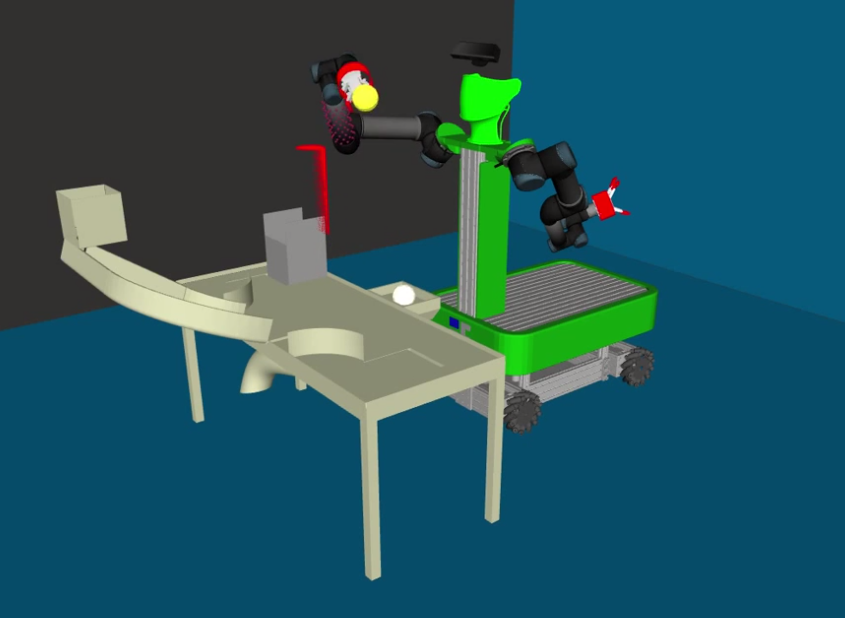
\includegraphics{chapters/doa/images/tomm_simulation.png}}\\[-10pt]
\caption[]{Orange sorting scenario in simulation.}
\label{fig:TOMMSimulation}
\end{figure}
The combined use of a reactive motion planner and a hierarchical reactive SoT controller with skin data makes it a good candidate for applying dynamical obstacle avoidance in factory environments. A video result of the same is available \href{https://youtu.be/uLStjR7mpOI}{\textcolor{blue}{here}}. Though it is tested in simulation, an experimental verification on a real robot setup with 3d cameras is quite essential to qualify the proposed framework as a promising technology. But the collision avoidance is tested on a UR robot with skin sensors to verify the local reactivity of the controller. 

\subsection{Experiments in a UR5 robot}

\begin{figure}[H]
\centering
{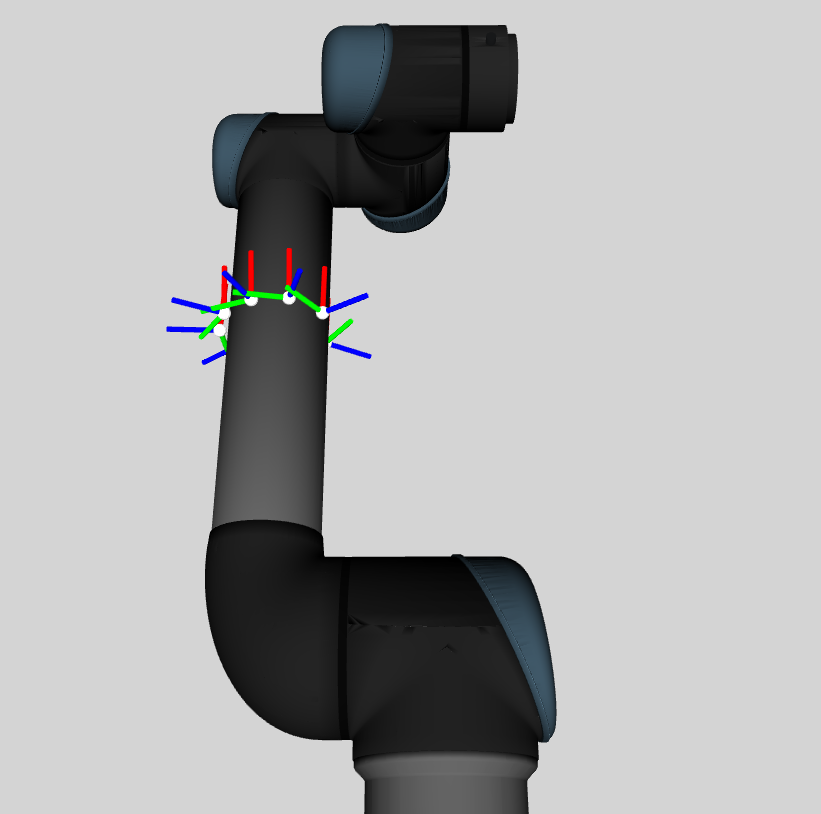
\includegraphics[width=6.5cm,height=6cm]{chapters/doa/images/delft/ring_sensors.png}}
\caption{Sensor Ring on the Upper Arm}
\label{fig:ringsensors}
\end{figure}

The reactive collision avoidance is experimentally verified on the UR5 robot with the skin sensor setup. The skin sensor network  consists of approximately 300 cells in total covering the entire surface of the UR5 robot arm. Though it is interesting to model all the skin cell constraints to be resolved by the controller, it is practically impossible to solve all the inequality constraints using the current state of the art solver due to computational constraints. A proper approximation is necessary to minimize the number of inequality constraints fed to the solver at every control cycle. In the set of preliminary experiments conducted, we defined a skin sensor ring in the upper arm as shown the figure \ref{fig:ringsensors} and collision avoidance constraints are applied only on this ring. The ring's central location on the arm gives symmetry which allows to sense information from all the directions. Another note is that the reactive replanning component is not tested in these experiments because of practical unavailability of the physical setup. 

Predefined trajectories are executed for different obstacle positions with and without collision avoidance task to verify the validity of the collision avoidance mechanism implemented. Three robot positions are chosen: Home position, Pick position and Place position. The repetitiveness of these tests on different object locations is to justify the symmetry of the ring and the robustness of the controller. There is also a complete manipulation scenario shown in the end of experiments to illustrate the practical use of the implementation. This component was successfully integrated in the final project demonstration of Factory-in-a-day which ran for more than 20 minutes robustly without any controller failure though it is possible in the most optimization based solvers. The simplicity of the approach and the practical relevance makes it a best candidate for being used in industries. 

\begin{figure}[H]
\centering
\begin{subfigure}
[Home Position]{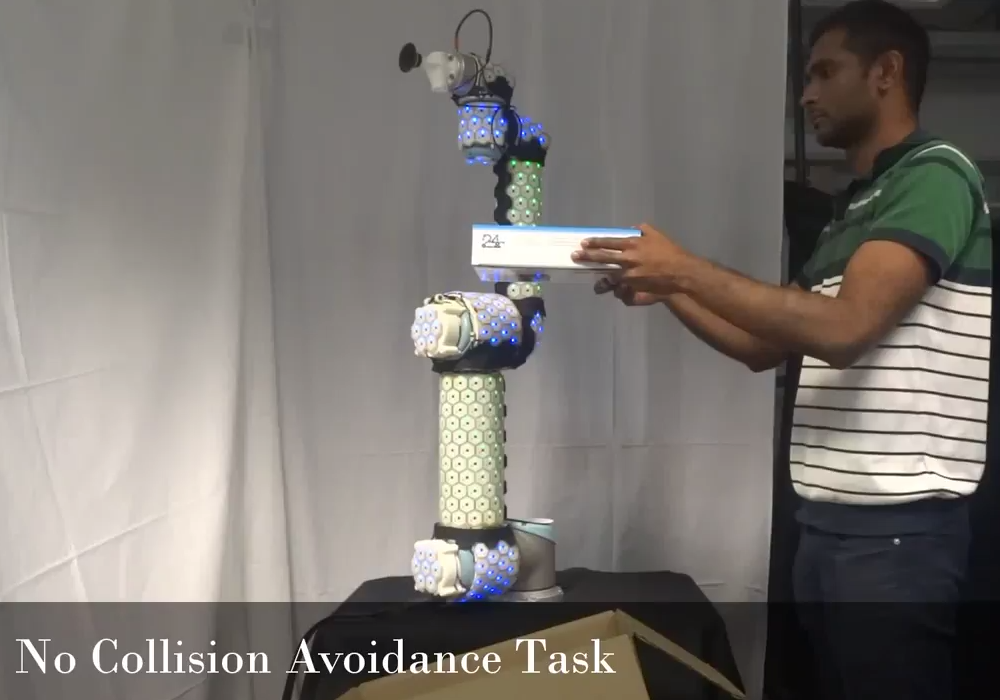
\includegraphics[width=6.5cm,height=6cm]{chapters/doa/images/delft/test_home2pick/cropped/test0_0-cropped.png}}
\end{subfigure}
\begin{subfigure}
[Colliding with Obstacle]{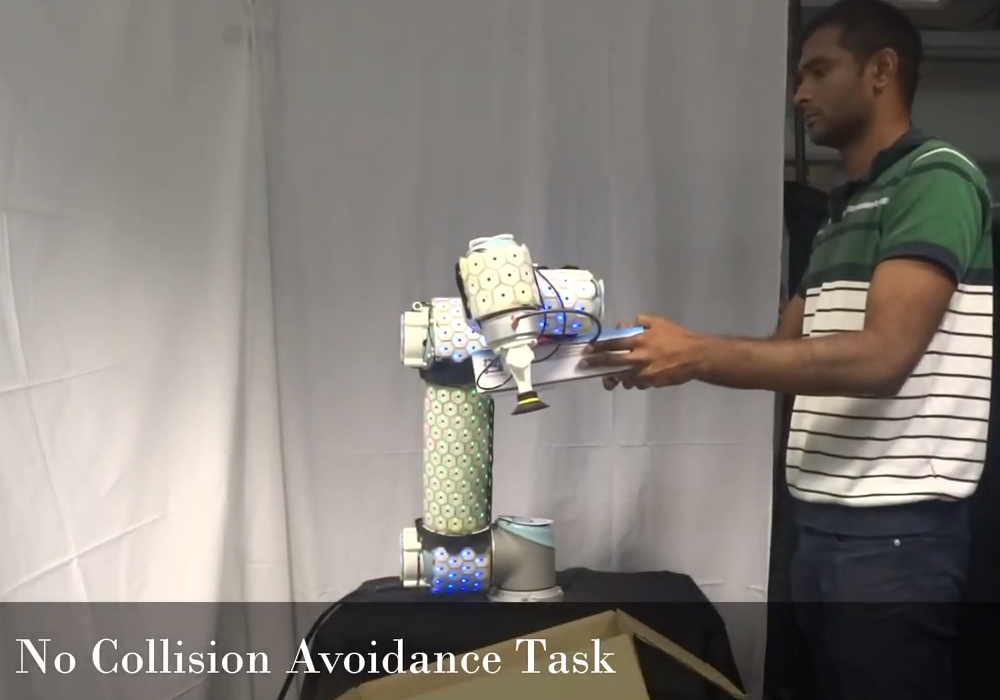
\includegraphics[width=6.5cm,height=6cm]{chapters/doa/images/delft/test_home2pick/cropped/test0_1-cropped.png}}
\end{subfigure}
\begin{subfigure}
[Avoiding Local Collisions]{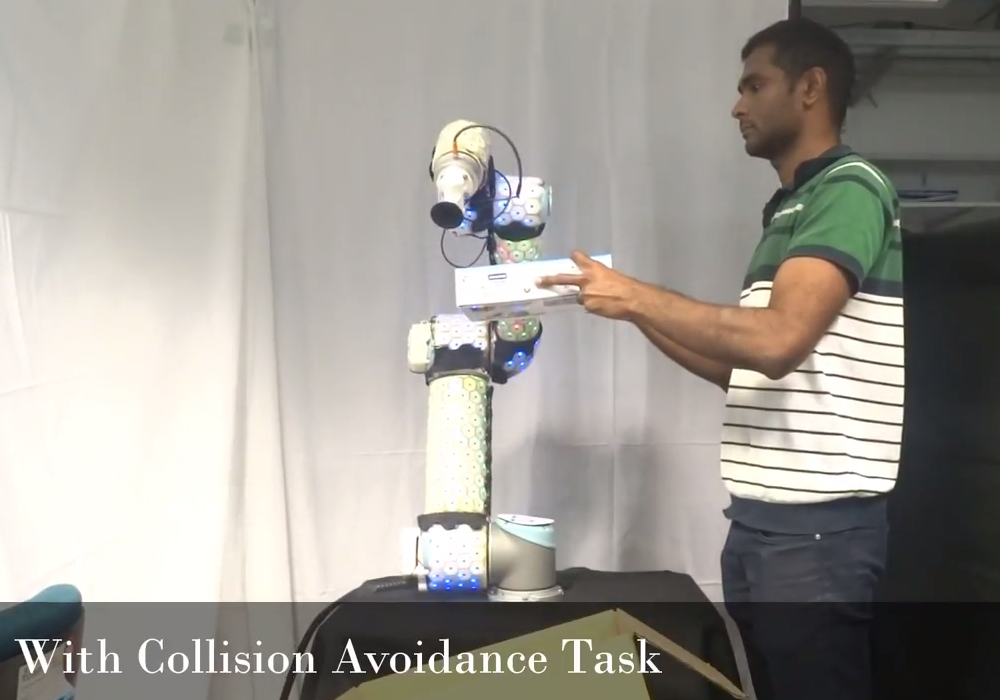
\includegraphics[width=6.5cm,height=6cm]{chapters/doa/images/delft/test_home2pick/cropped/test0_2-cropped.png}}
\end{subfigure}
\begin{subfigure}
[Place Position after avoiding Collisions]{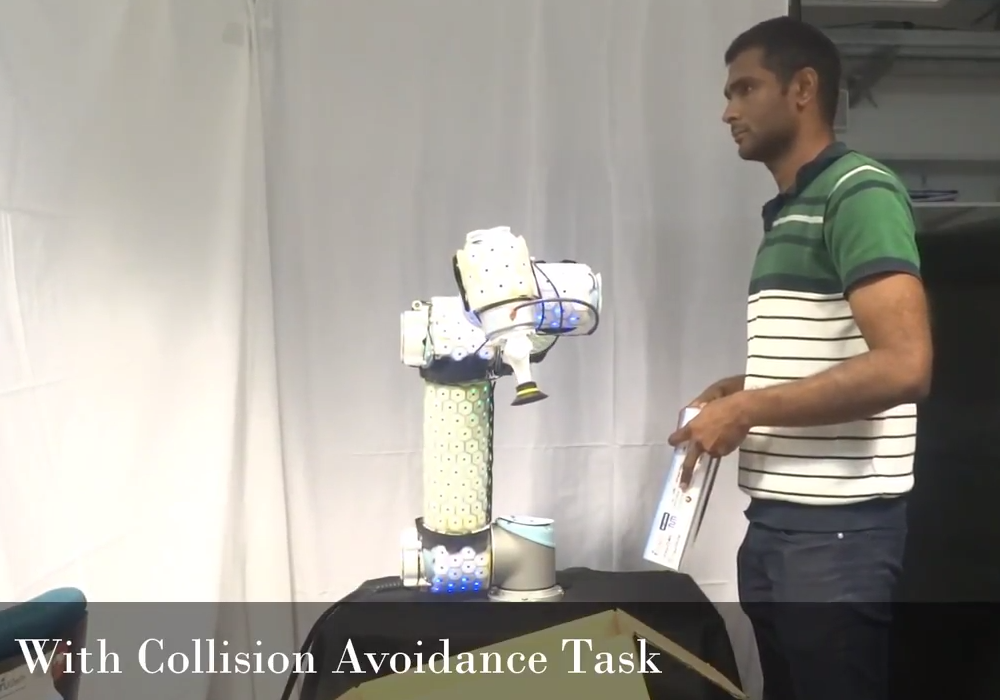
\includegraphics[width=6.5cm,height=6cm]{chapters/doa/images/delft/test_home2pick/cropped/test0_3-cropped.png}}
\end{subfigure}
\caption{Test 1: Trajectory execution from home to pick location with and without collision avoidance task in the controller stack. (b) shows the collision with the obstacle without the ability to avoid collision. (b) shows the collision avoidance of the arm though it gets stuck in the local minima but reaches the goal after the obstacle is removed.}
\label{fig:h2ptest1}
\end{figure}
The experimental validation done on the robot can be seen in these videos demonstrating three scenarios : \href{https://goo.gl/LVbQZz}{\textcolor{blue}{home to pick}}, \href{https://goo.gl/7jCqzA}{\textcolor{blue}{pick to place}}, \href{https://goo.gl/GP8KAA}{\textcolor{blue}{place to home}}. As it can be seen, a box is used as an obstacle to interrupt the executed path. Three tests are conducted at different obstacle locations introducing variability in the environment with these obstacles. Though there are many tests conducted, let us focus on certain tests and the behavior to illustrate the performance of the controller. The figure \ref{fig:h2ptest1} shows the test executing a trajectory from home to pick location with a fixed obstacle location as shown. (a) shows the initial state of the robot which is the home position and (b) shows the trajectory execution without any collision avoidance task to differentiate with the behavior generated by the controller with collision avoidance task. The robot evading collisions and its inability to reach the goal because of the object can be seen in (c) and (d). It gets stuck in local minima but manages to reach the goal after the object is removed. 

\begin{figure}[H]
\centering
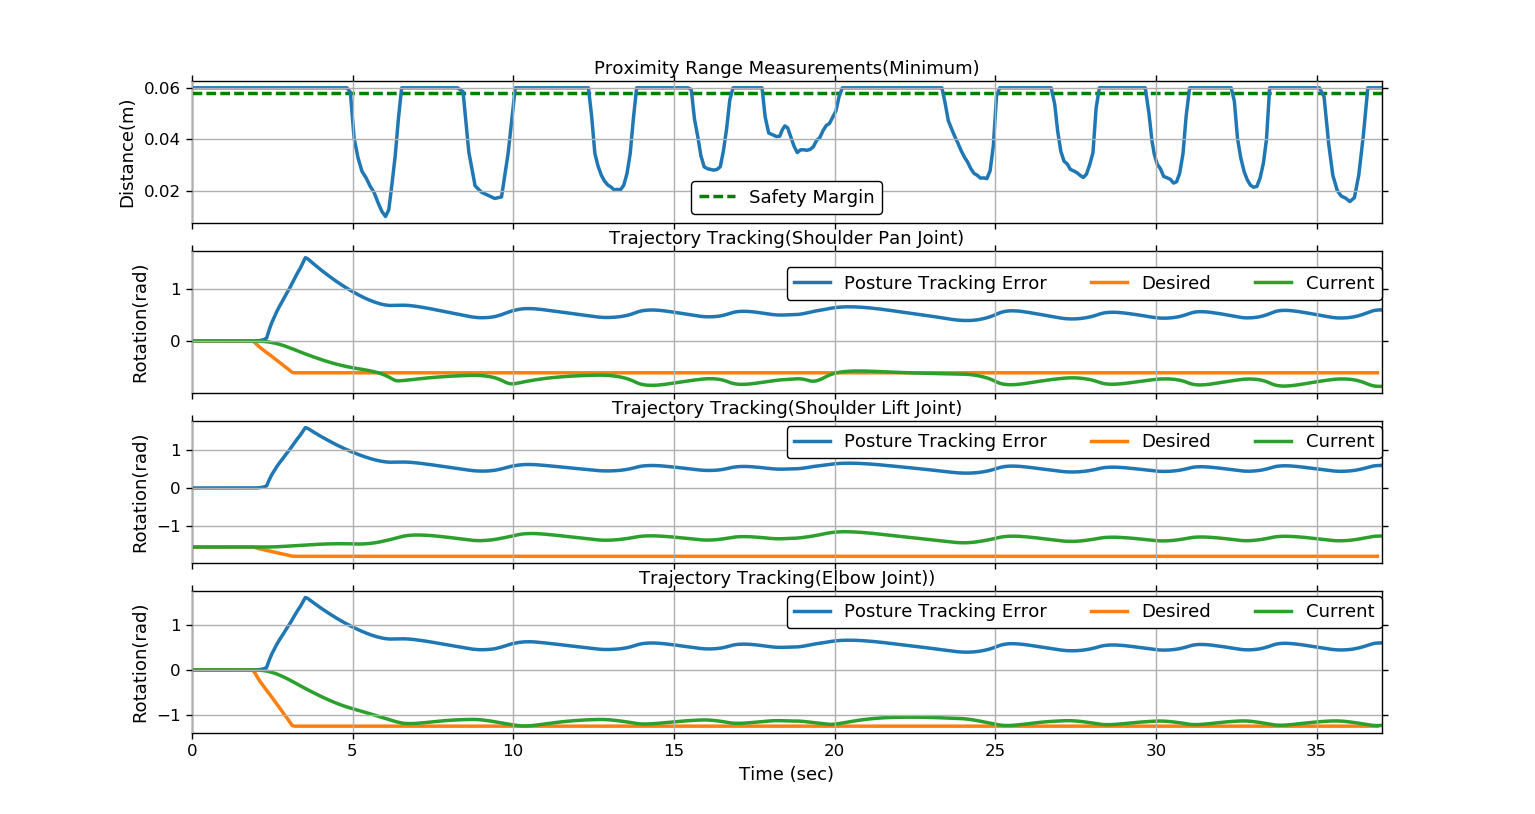
\includegraphics[width=18cm,height=13cm,center]{chapters/doa/images/delft/test_home2pick/plot_0.png}
\caption{Test 1: Plot during a Home to Pick Trajectory Execution: (1) shows the the min of range measurements from 8 skin sensor cells showing the vicinity of obstacles to the upper arm. (2),(3) and (4) shows the disturbances in the trajectory tracking when an obstacle is in the vicinity. The Posture tracking error doesn't settle to zero because of the local minima it encounters, resulting in continuous oscillations trying to go across the obstacle with a hope the obstacle will move away'}
\label{Home2Pick:test1}
\end{figure}
The plot in \ref{Home2Pick:test1}, \ref{Home2Pick:test2} shows the evolution of the trajectory tracking error and the proximity range measurements during the execution of a trajectory from home to pick with two obstacle locations respectively. The minimum of the proximity measurements of 8 cells is taken to show in the plots showing the presence of the obstacle close to the arm. The trajectory tracking error is the 2-norm of the current state of the robot and the posture command of the trajectory sequencer fed to posture task stacked in the solver.  Along with the trajectory error, the three major joints: shoulder pan, shoulder lift and the elbow joint states are plotted with the desired state to show the perturbations in response to the obstacle close to the arm. In both the plots, it can be observed that the trajectory tracking error increases rapidly irrespective of the obstacles at a proximity distance above the safety margin. This is because of the formulation as shown in \ref{eq:dd_ineq}, the collision avoidance task constrains the velocity of the skin cell based on the difference between the safety margin and the measured range. From the plots it can be observed, the difference is around 2 millimeter when there is no object close to the arm. The skin sensor range information is saturated to 6cm as the measurements above 6cm are highly nonlinear and unreliable. The 2mm difference along with smaller task gains reduces the speed of the robot. Though the saturation value can be adjusted to improve the speed of the robot behavior, the plots correspond to a non-ideal setting but still shows a robust collision avoidance. 


\begin{figure}[H]
\centering
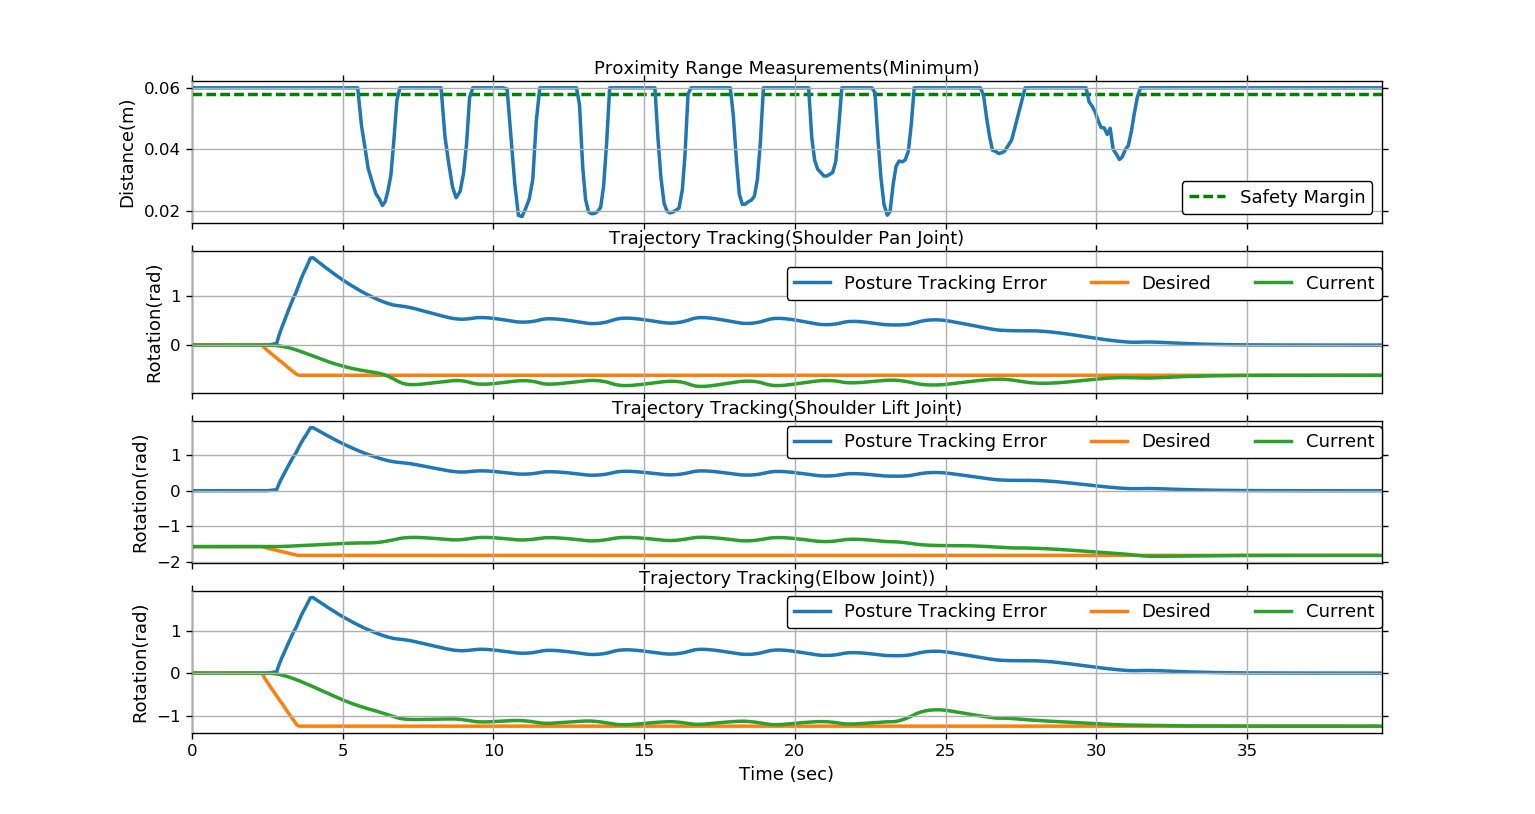
\includegraphics[width=18cm,height=13cm,center]{chapters/doa/images/delft/test_home2pick/plot_1.png}
\caption{Test 2: Plot during a Home to Pick Trajectory Execution: (1) shows the the min of range measurements from 8 skin sensor cells showing the vicinity of obstacles to the upper arm. (2),(3) and (4) shows the disturbances in the trajectory tracking when an obstacle is in the vicinity. The Posture tracking error settles to zero because the resulting deformation in trajectory was sufficient to evade obstacles and still achieve the goal.}
\label{Home2Pick:test2}
\end{figure}

In both the plots \ref{Home2Pick:test1} and \ref{Home2Pick:test2} , the disturbances in trajectory tracking when an obstacle is in the vicinity. In \ref{Home2Pick:test1}, the posture tracking error doesn’t settle to zero because of the local minima it encounters, resulting in continuous oscillations trying to go across the obstacle with a hope the obstacle will move away. In \ref{Home2Pick:test1}, the posture tracking error settles to zero because the resulting deformation in trajectory was sufficient to evade obstacles and still achieve the goal. In contrast to the previous plots, the plot \ref{Home2Pick:nocollision} shows the trajectory execution without collision avoidance task in the stack. As it can be seen in the video and in the plot, the trajectory execution was not affected while the arm literally goes across the obstacles which can be seen in the closeness of arm with the obstacles. The shoulder pan \& lift joint, elbow joint trajectory tracking is smooth without any disturbances like we saw in the previous plots validating the controller(with collision avoidance task) of taking actions in response to the obstacles in the vicinity.

\begin{figure}[H]
\centering
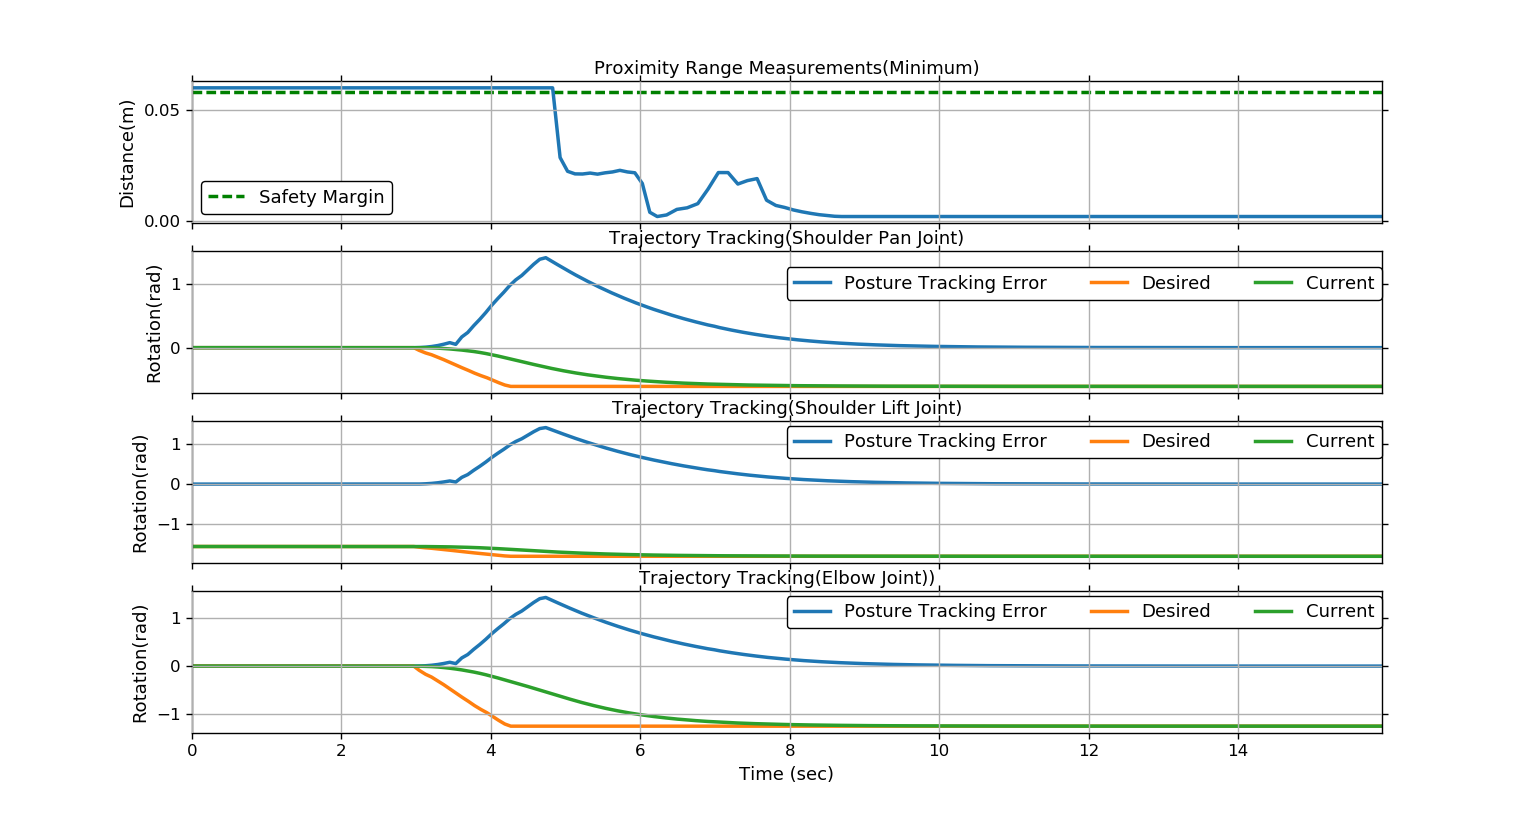
\includegraphics[width=18cm,height=13cm,center]{chapters/doa/images/delft/test_home2pick/plot_0_nocollision.png}
\caption{Test 1: Plot during a Home to Pick Trajectory Execution with no Collision Avoidance task in the Stack: (1) shows the the min of range measurements from 8 skin sensor cells showing the vicinity of obstacles to the upper arm. The sensor range drops close to zero showing the obstacle literally touching the robot. (2),(3) and (4) shows no disturbances in the trajectory tracking when an obstacle is in the vicinity. The Posture tracking error settles to zero after reaching the goal just by hitting the obstacle obviously because of no awareness.}
\label{Home2Pick:nocollision}
\end{figure}

The figure \ref{fig:p2ptest3} shows the test executing a trajectory from pick to place location with a fixed obstacle location as shown. (a) shows the initial state of the robot which is the pick position and (b) shows the trajectory execution without any collision avoidance task to differentiate with the behavior generated by the controller with collision avoidance task. The robot evading collisions and its ability to reach the goal by deforming the trajectory as seen in (c),(d) and (e) to reach (f). Similar natural behaviors can be seen in the rest of the videos referred previously.

\begin{figure}[H]
\centering
\begin{subfigure}
[Initial State - Pick Position]{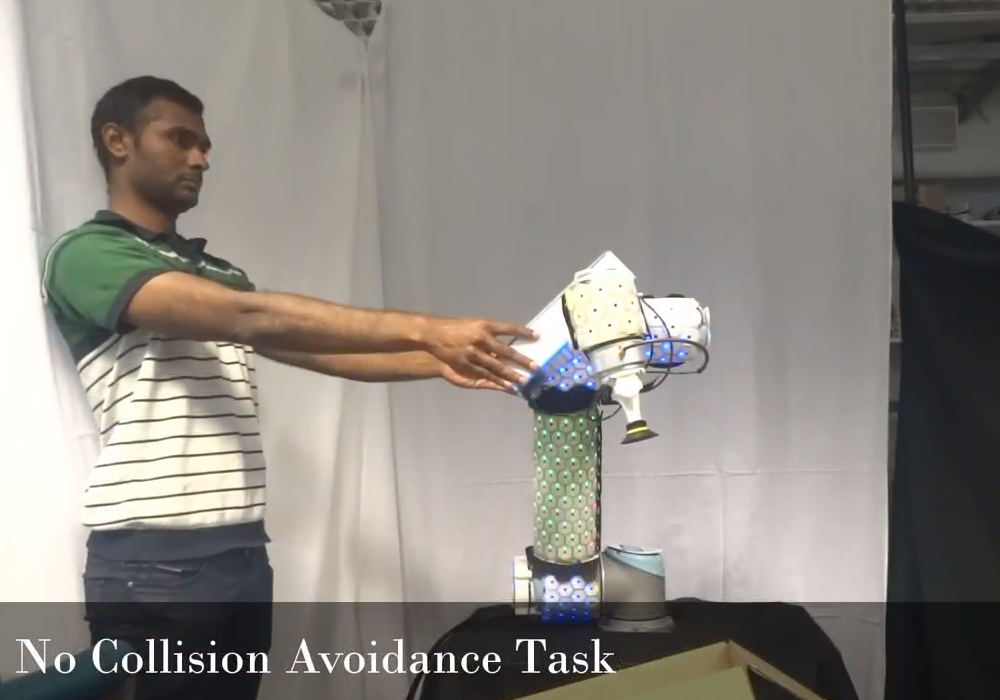
\includegraphics[width=6.5cm,height=6cm]{chapters/doa/images/delft/test_pick2place/cropped/test2_0-cropped.png}}
\end{subfigure}
\begin{subfigure}
[Colliding with Obstacle]{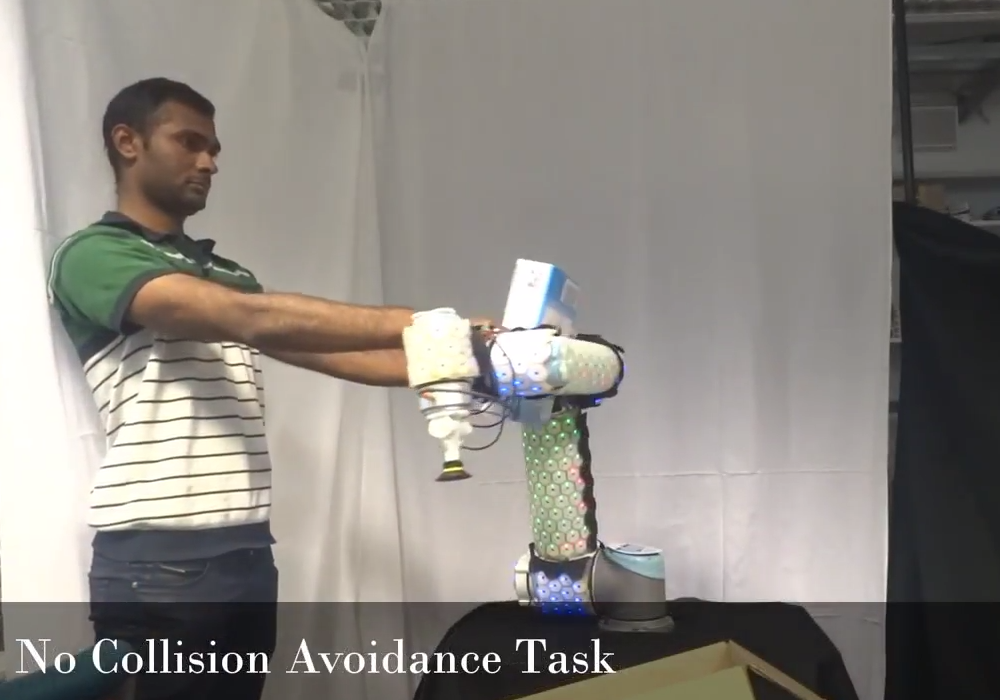
\includegraphics[width=6.5cm,height=6cm]{chapters/doa/images/delft/test_pick2place/cropped/test2_1-cropped.png}}
\end{subfigure}
\begin{subfigure}
[Avoiding Local Collisions 1/3]{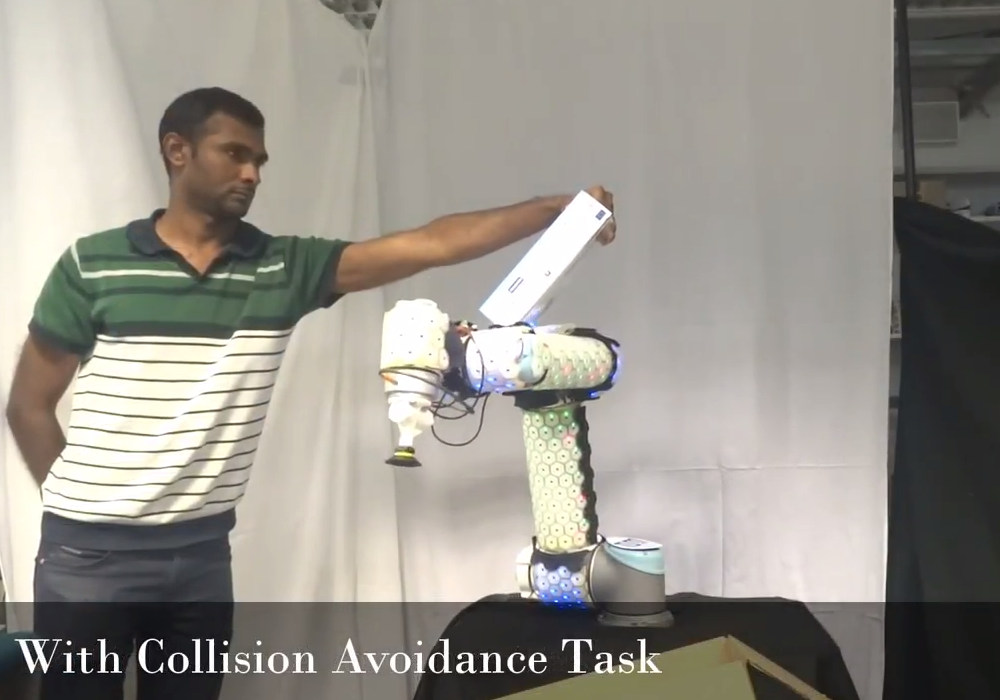
\includegraphics[width=6.5cm,height=6cm]{chapters/doa/images/delft/test_pick2place/cropped/test2_2-cropped.png}}
\end{subfigure}
\begin{subfigure}
[Avoiding Local Collisions 2/3]{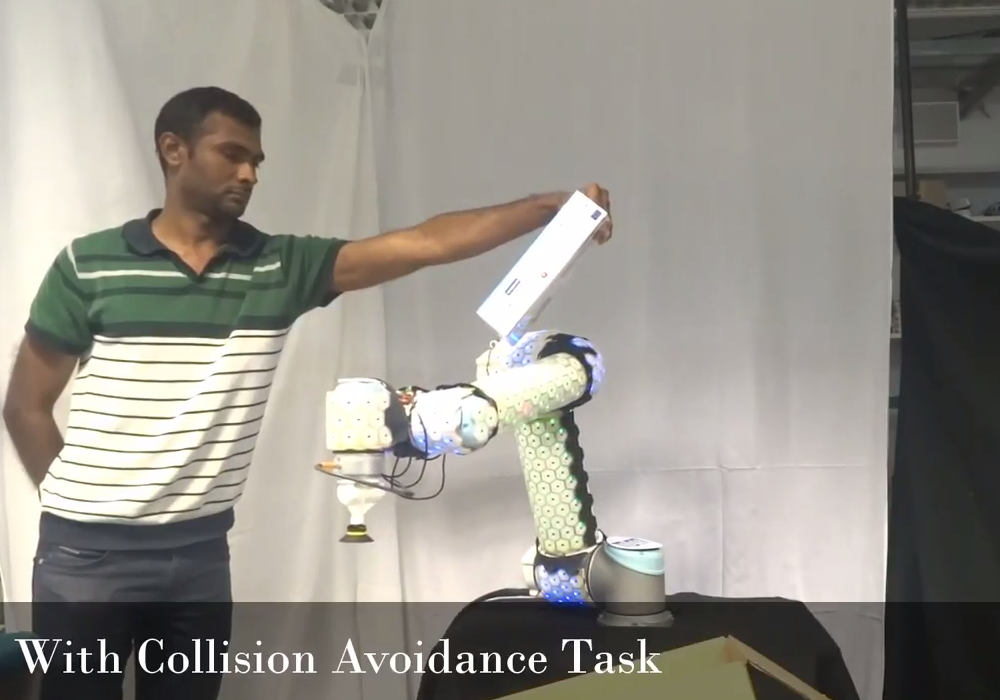
\includegraphics[width=6.5cm,height=6cm]{chapters/doa/images/delft/test_pick2place/cropped/test2_2_1-cropped.png}}
\end{subfigure}
\begin{subfigure}
[Avoiding Local Collisions 3/3]{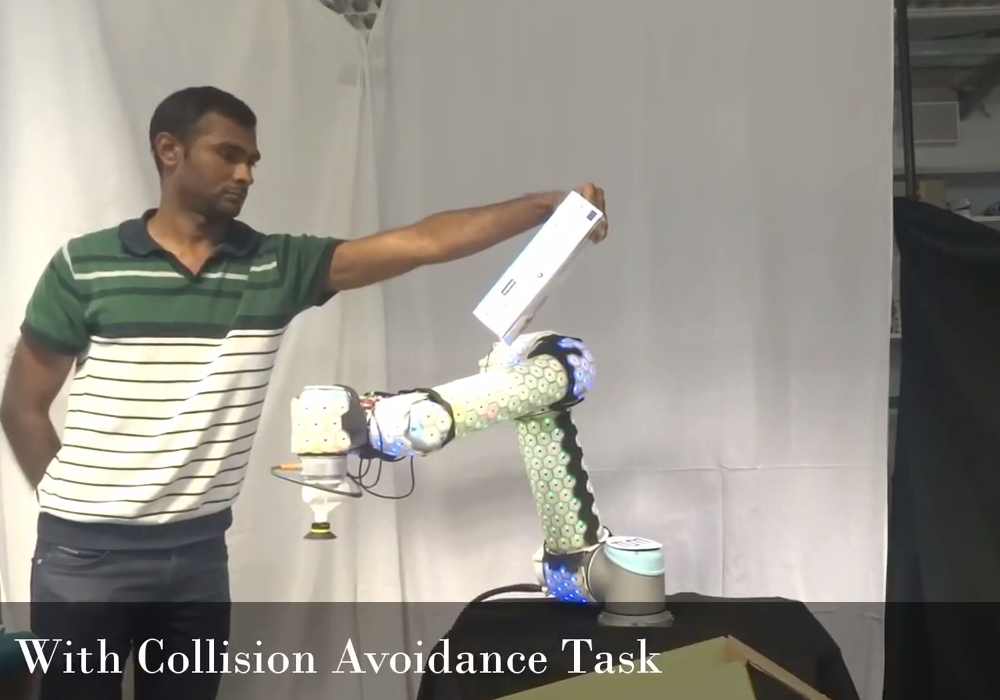
\includegraphics[width=6.5cm,height=6cm]{chapters/doa/images/delft/test_pick2place/cropped/test2_2_2-cropped.png}}
\end{subfigure}
\begin{subfigure}
[Final State - Place Position]{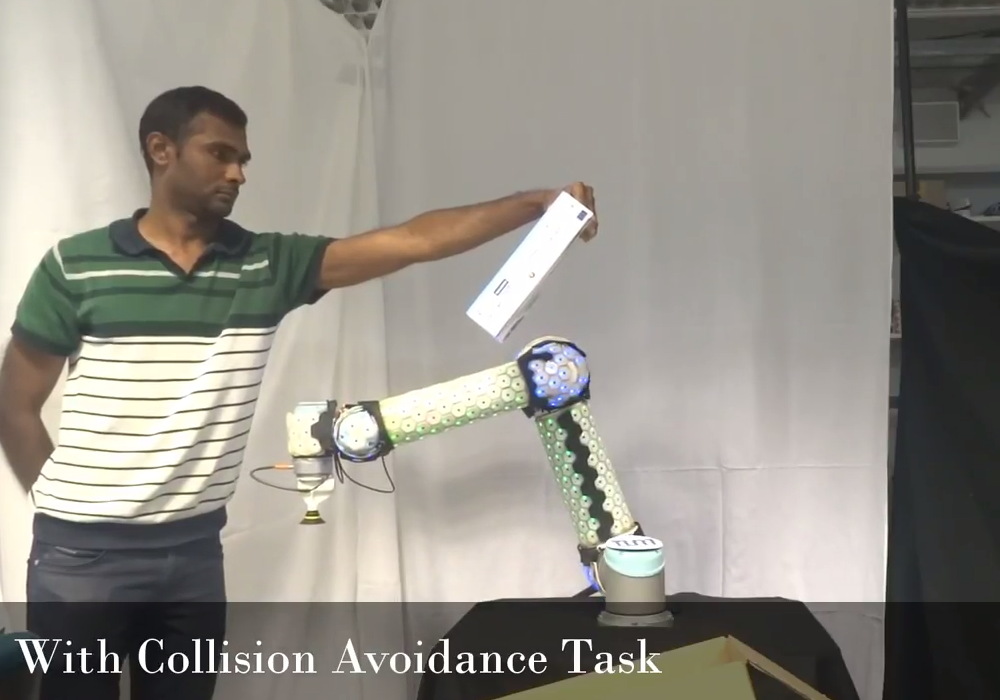
\includegraphics[width=6.5cm,height=6cm]{chapters/doa/images/delft/test_pick2place/cropped/test2_3-cropped.png}}
\end{subfigure}
\caption{Trajectory execution from pick to place location with and without collision avoidance task in the controller stack. (b) shows the collision with the obstacle without the ability to avoid collision. (b) shows the collision avoidance of the arm with a deformation in trajectory that allows the reach the goal with ease.}
\label{fig:p2ptest3}
\end{figure}

The reactive collision avoidance component after proper tuning is applied on a complete manipulation scenario involving multiple sequences of pick and place operations of boxes and shaving cans using a suction gripper in the end effector. The robot controller still holds the same ring of collision constraints in the upper arm for simplicity. The demonstration video is shown in this link \href{https://goo.gl/PLbKdb}{\textcolor{blue}{here}} with snapshots shown in . 

\begin{figure}[H]
\centering
\begin{subfigure}
[Grasping with a suction gripper]{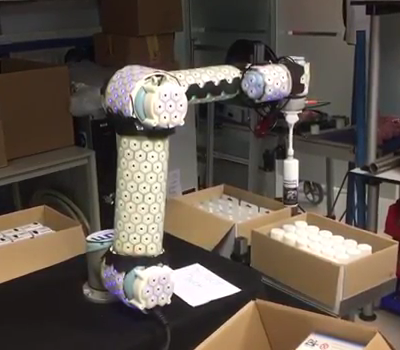
\includegraphics[width=6.5cm,height=6cm]{chapters/doa/images/delft/complete/suckstill-cropped.png}}
\end{subfigure}
\begin{subfigure}
[Avoiding Obstacles]{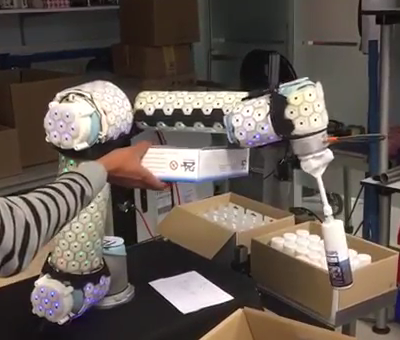
\includegraphics[width=6.5cm,height=6cm]{chapters/doa/images/delft/complete/avoiding-cropped.png}}
\end{subfigure}
\caption{Illustrating obstacle avoidance while picking and placing small objects using a suction gripper. The full scenario video can be seen in this \href{https://goo.gl/PLbKdb}{\textcolor{blue}{video}}.}
\label{fig:final_scenario}
\end{figure}

\begin{figure}[H]
\centering
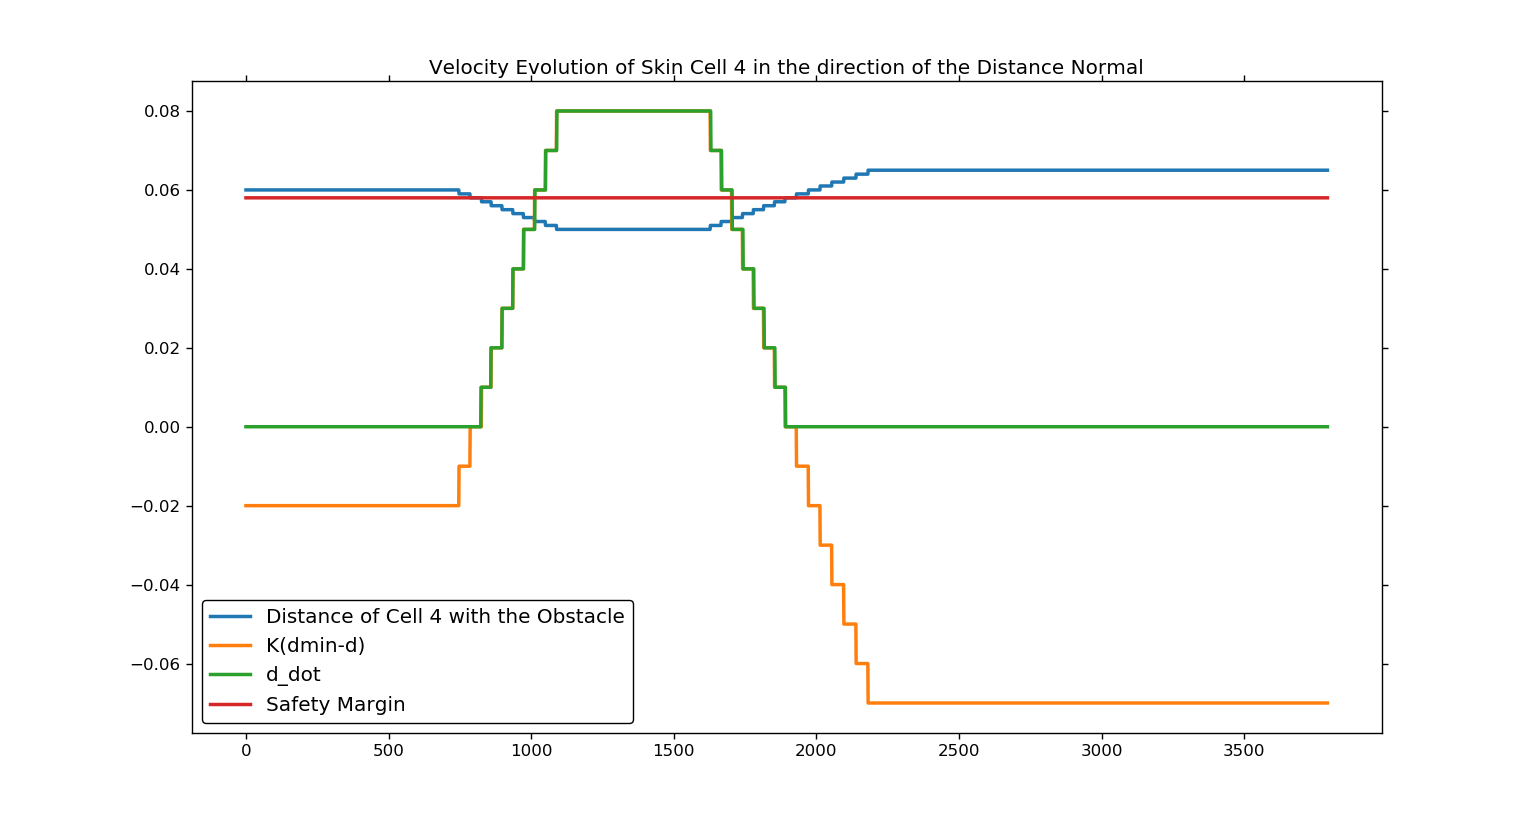
\includegraphics[width=18cm,height=8cm,center]{chapters/doa/images/delft/plot_satisfy.png}
\caption{Plot showing the evolution of a skin cell velocity satisfying the \ref{eq:dd_ineq} when the other cells have no obstacles in the vicinity.}
\label{fig:plotsatisfy}
\end{figure}

Another interesting aspect of the controller is the ability to compromise with the collision constraint inequalities in case the modeled constraint is not feasible without breaking the solver making the controller reliable. The plot \ref{fig:plotsatisfy} shows the change in velocity of a specific skin cell in response to changing obstacle in the vicinity. This plot is generated by simulating a distance signal to cell number 4 (among the 8 cells) around the safety margin while keeping the other skin cell values equal to 0.6 which is 10 times far away from the safety margin. This shows a practical feasibility of the goal thus resulting in a behavior inline with the formulated collision avoidance constraint in \ref{eq:dd_ineq}. 

But when we have a situation where the obstacles are around the arm in all directions within or beyond the safety margin, the controller compromises with the collision avoidance constraint as shown in the plot. This might look like a design issue but this is purely because of the nature of the HQP solver which compromises with the goal to achieve the maximum possible without breaking the controller or generating bad motion behaviors making it reliable. 

\begin{figure}[H]
\centering
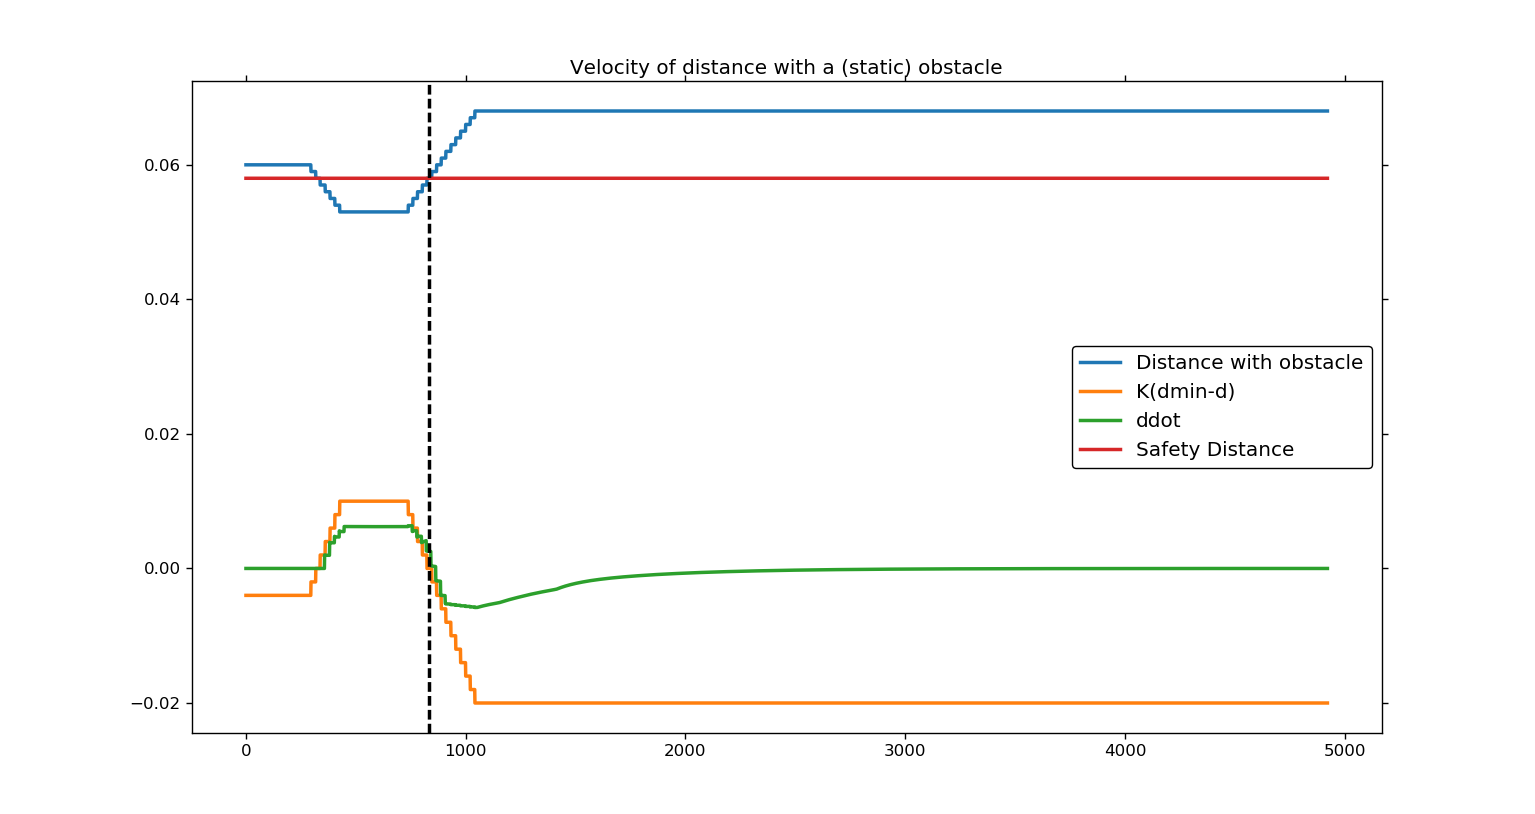
\includegraphics[width=18cm,height=8cm,center]{chapters/doa/images/delft/plot_unsatisfy.png}
\caption{Plot showing the evolution of a skin cell velocity not satisfying the \ref{eq:dd_ineq} when the other cells have obstacles in the vicinity but not inside the safety margin. The other skin cells are simulated to measure 6cm which is just 2mm from the safety margin. This constrains the upper arm in achieving a skin cell velocity satisfying the \ref{eq:dd_ineq} as the control believes there is an obstacle still around hence resulting in safer motions.}
\label{fig:plot_unsatisfy}
\end{figure}






